\section{Mechanical Design}
\label{sec:mechanical}

The robot was modelled in SolidWorks. This section gives the layout, the mass properties and
what follows from them, the drive, the gripper and the placement of the sensors. Dimensions
and masses are those of the CAD model as exported for the simulation
(\code{trident.urdf.xacro}); none of them was measured on the printed robot.

\subsection{Layout}
\label{sec:layout}
The chassis is a single printed plate of $180\times150\times6\unit{mm}$
(\cref{fig:cad-views}). Two N20 gearmotors are fixed under its rear edge and drive two
wheels of 22\unit{mm} radius, 195.5\unit{mm} apart. A ball caster under the plate, 85\unit{mm}
ahead of the axle, is the third support. The servo of the gripper stands on the plate near
the front edge, with its shaft pointing down through the plate, and the two jaws turn in a
horizontal plane below the plate and reach forward of it. The infrared array hangs under the
plate between the axle and the caster, and the depth camera sits in a holder on a post at the
left side of the plate. The battery and the control electronics occupy the rear of the plate
above the axle.

\begin{figure}[htbp]
  \centering
  \begin{subfigure}[b]{0.30\linewidth}
    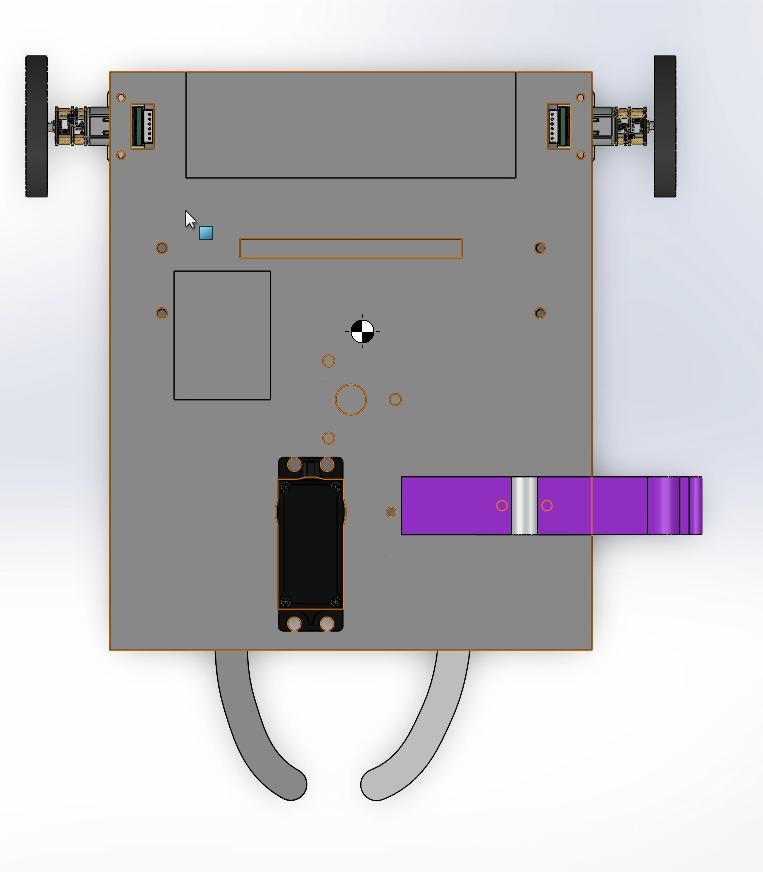
\includegraphics[width=\linewidth]{cad_top.png}
    \caption{Top}
  \end{subfigure}\hfill
  \begin{subfigure}[b]{0.30\linewidth}
    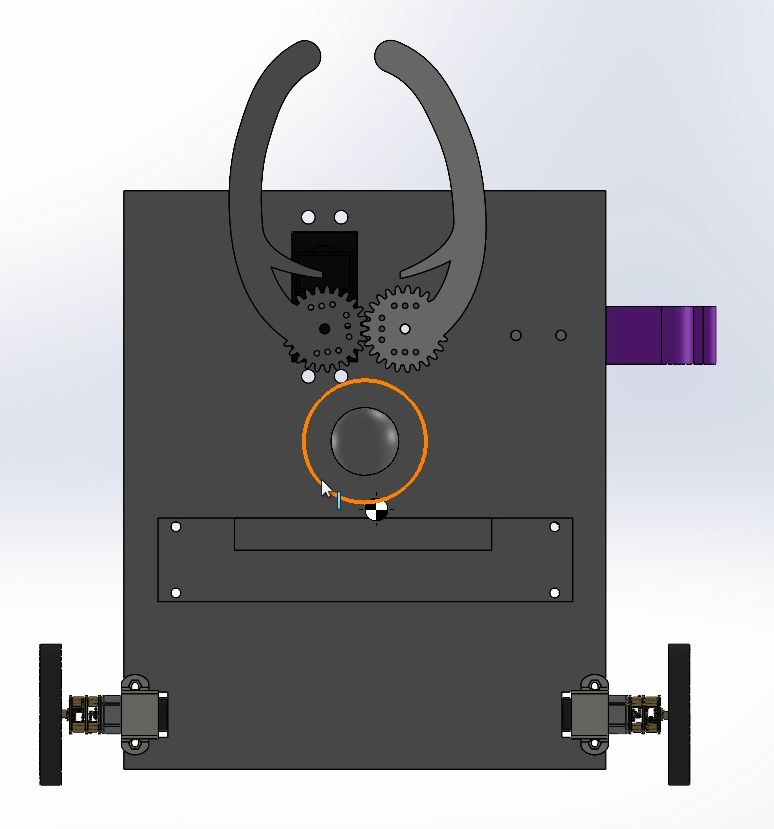
\includegraphics[width=\linewidth]{cad_bottom.png}
    \caption{Bottom}
  \end{subfigure}\hfill
  \begin{subfigure}[b]{0.36\linewidth}
    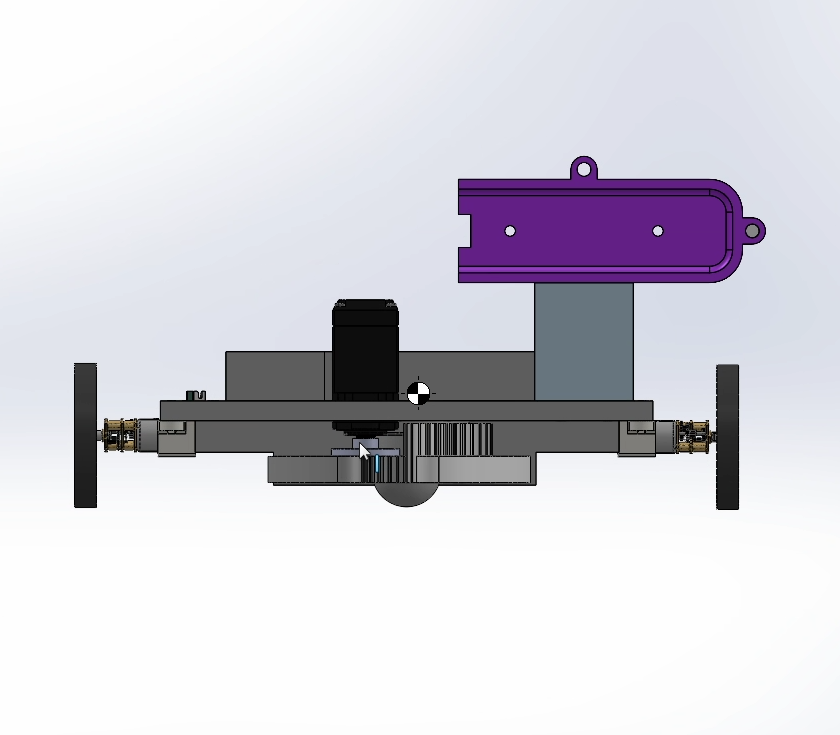
\includegraphics[width=\linewidth]{cad_front.png}
    \caption{Front}
  \end{subfigure}
  \caption{CAD model of Version 2. The black and white disc marks the centre of mass
  calculated by the CAD program. In the bottom view the caster is the dome at the centre and
  the two gears of the gripper are in front of it.}
  \label{fig:cad-views}
\end{figure}

\Cref{tab:dimensions} lists the principal dimensions.

\begin{table}[htbp]
  \centering
  \caption{Principal dimensions of the robot, from the CAD model.}
  \label{tab:dimensions}
  \begin{tabular}{@{}ll@{}}
    \toprule
    Quantity & Value \\
    \midrule
    Chassis plate & $180\times150\times6\unit{mm}$ \\
    Wheel radius, wheel separation & 22\unit{mm}, 195.5\unit{mm} \\
    Caster ahead of the axle & 85.0\unit{mm} \\
    Jaw pivots: ahead of the axle, apart & 120.0\unit{mm}, 25.0\unit{mm} \\
    Reach of a jaw from its pivot & 90\unit{mm} \\
    Infrared array: ahead of the axle, above the floor & 48\unit{mm}, 7.4\unit{mm} \\
    Infrared channels, pitch & 8, 15\unit{mm} \\
    Camera: above the floor, left of the centre line & 85\unit{mm}, 54\unit{mm} \\
    Total mass of the model & 0.64\unit{kg} \\
    \bottomrule
  \end{tabular}
\end{table}

\subsection{Mass Properties and Their Consequences}
\label{sec:mass}
The first requirement of \cref{sec:evolution} concerns the centre of mass. The CAD export
gives a mass and a centre of mass for every part, so the requirement can be checked
(\cref{tab:mass}). The origin is the midpoint of the axle, $x$ points forward and $y$ to
the left.

\begin{table}[htbp]
  \centering
  \caption{Mass budget of the model. The chassis assembly is the plate with the motors, the
  servo and the blocks that stand for battery and electronics in the CAD model.}
  \label{tab:mass}
  \begin{tabular}{@{}lrrr@{}}
    \toprule
    Part & Mass [g] & $x$ [mm] & $y$ [mm] \\
    \midrule
    Chassis assembly & 425.6 & 50.2 & $-5.5$ \\
    Depth camera (D435) & 72.0 & 129.5 & 54.3 \\
    Camera holder & 58.8 & 116.2 & 58.1 \\
    Jaws (two) & 34.8 & 146.4 & 0.3 \\
    Wheels (two) & 20.2 & 0.0 & 0.0 \\
    Infrared array & 20.0 & 49.7 & 0.0 \\
    Caster & 8.9 & 85.0 & 0.0 \\
    \midrule
    Robot & 640.3 & 69.3 & 7.8 \\
    \bottomrule
  \end{tabular}
\end{table}

\paragraph{Wheel loads.} The centre of mass lies 69.3\unit{mm} ahead of the axle and the
caster 85.0\unit{mm}. With $W=mg=6.28\unit{N}$, the caster at $x_k$ and the centre of mass
at $x_c$, the static loads are
\begin{equation}
  N_k = W\,\frac{x_c}{x_k} = 5.12\unit{N}, \qquad
  N_w = W\Bigl(1-\frac{x_c}{x_k}\Bigr) = 1.16\unit{N},
  \label{eq:loads}
\end{equation}
where $N_w$ is the sum over both wheels. The centre of mass is inside the support triangle,
as required. It lies closer to the caster than to the axle: in the model the wheels carry 18\,\% of the
weight and the caster 82\,\%. The camera with its holder, 131\unit{g} at the front of the
plate, and the jaws are responsible. The CAD views of \cref{fig:cad-views} agree with this:
the centre-of-mass mark lies next to the caster.

\paragraph{Traction limit.} The wheel load bounds the force that the wheels can transmit.
With a coefficient of friction $\mu$ between tyre and floor,
\begin{equation}
  a_{\max} = \frac{\mu N_w}{m} = \mu g\Bigl(1-\frac{x_c}{x_k}\Bigr) = 1.8\,\mu\unit{m/s^2},
  \label{eq:traction}
\end{equation}
so that even with $\mu=1$ the robot cannot accelerate or brake at more than
1.8\unit{m/s^2} without slip. This limit is visible in the simulation. With no limit on the
deceleration, the wheels of the simulated robot stopped at once on a stop command and the
robot skidded and turned; the drive is now limited to 1.0\unit{m/s^2}
(\cref{sec:sim-drive}). The force needed to slide a coin, by contrast, is small: a coin of
23\unit{g} with a friction coefficient of 0.35 resists with 0.08\unit{N}.

\paragraph{Tipping margin.} On three supports the robot tips about an edge of the support
triangle (\cref{fig:triangle}). The triangle is narrow at the caster, and the centre of mass
is both far forward and, because of the camera, 7.8\unit{mm} to the left. Its distance to
the left edge of the triangle is $d=6.7\unit{mm}$ and to the right edge 16.9\unit{mm}. With
the centre of mass at a height $h=42\unit{mm}$ above the floor, a horizontal acceleration
$a$ directed across the left edge tips the robot when $a>g\,d/h=1.6\unit{m/s^2}$. A braking
deceleration acts along $x$, at an angle to that edge, and tips the robot above
2.1\unit{m/s^2}. Both values are above the 1.0\unit{m/s^2} that the drive is allowed, but
the margin is a factor of two and not more.

\begin{figure}[htbp]
  \centering
  \begin{tikzpicture}[scale=0.42]
    % units: 10 mm. x forward is drawn upward, y left is drawn to the left.
    \draw[draw=ink!45, fill=panel] (-7.5,-1.7) rectangle (7.5,16.3);
    \node[note, anchor=south west] at (-7.5,-1.7) {plate};
    % wheels
    \fill[ink] (-10.1,-2.2) rectangle (-9.45,2.2);
    \fill[ink] (9.45,-2.2) rectangle (10.1,2.2);
    % support triangle
    \draw[cA, line width=0.9pt] (-9.777,0) -- (9.777,0) -- (0,8.5) -- cycle;
    \fill[cA] (0,8.5) circle (0.22);
    \node[note, anchor=west] at (0.4,8.9) {caster};
    \node[note, anchor=north] at (0,-0.1) {axle};
    % centre of mass
    \fill[cB] (-0.78,6.93) circle (0.25);
    \draw[draw=cB!60] (-0.5,7.05) -- (4.0,7.9);
    \node[note, anchor=west, text=cB] at (4.0,7.9) {centre of mass};
    \draw[cB, line width=0.6pt] (-0.78,6.93) -- (-1.22,7.44);
    \node[note, anchor=east, text=cB] at (-1.4,7.6) {6.7\,mm};
    % camera and gripper pivots
    \draw[draw=ink, fill=white] (-9.9,11.7) rectangle (-0.9,14.2);
    \node[note] at (-5.4,12.95) {camera};
    \fill[ink] (-1.25,12.0) circle (0.14);
    \fill[ink] (1.25,12.0) circle (0.14);
    \node[note, anchor=west] at (1.6,12.0) {jaw pivots};
    % IR array
    \draw[draw=ink, fill=white] (-5.25,4.6) rectangle (5.25,5.0);
    \node[note, anchor=west] at (5.5,4.8) {IR array};
    % axes
    \draw[->] (15,0) -- (15,3) node[note, right] {$x$};
    \draw[->] (15,0) -- (12,0) node[note, below] {$y$};
    % scale
    \draw[|-|] (-7.5,-3.2) -- (7.5,-3.2);
    \node[note, below] at (0,-3.3) {150\,mm};
  \end{tikzpicture}
  \caption{Support triangle of the two wheels and the caster, seen from above, to scale.
  The centre of mass of the model lies inside it, 16\unit{mm} behind the caster and
  6.7\unit{mm} from the left edge.}
  \label{fig:triangle}
\end{figure}

\paragraph{What this means for the design.} The layout meets its requirement, and the
analysis shows where it can be improved. Two changes would raise the wheel load and the
tipping margin: moving the caster forward, towards the gripper pivots, which widens the
triangle around the centre of mass and transfers load to the wheels; and mounting the
camera on the centre line, which removes the lateral offset.
Two reservations apply. The masses are CAD values, and the blocks that stand for the
battery and the electronics need not carry their true mass, so the real centre of mass may
lie further back than \cref{tab:mass} says. And the printed robot has not been weighed
on its three supports, which would settle the question in a few minutes.

\subsection{Drive}
\label{sec:drive}
The robot is a differential drive. With wheel radius $r$, wheel separation $b$ and wheel
speeds $\omega_l$, $\omega_r$, the forward speed and the turn rate are
\begin{equation}
  v = \frac{r}{2}(\omega_r+\omega_l), \qquad \omega = \frac{r}{b}(\omega_r-\omega_l).
  \label{eq:diffdrive}
\end{equation}
N20 gearmotors were chosen because motors of higher torque do not fit under a plate of this
size. The simulation assumes a variant with a no-load speed of 300\unit{rpm} at
6\unit{V} and a stall torque of 0.05\unit{N\,m} at the wheel; both are placeholders in the
model and have to be replaced by the data of the motors fitted. On these values the robot
has a top speed of $r\,\omega=0.69\unit{m/s}$, and the mission uses at most
0.20\unit{m/s}, less than a third of it. The two motors together can push with
4.5\unit{N} at stall, about four times the 1.16\unit{N} that the wheels can transmit by
\cref{eq:loads}. The drive is therefore limited by traction and not by torque, which is a
further reason to move load onto the wheels.

The wheels are narrow, and the caster is a ball that slides. In the simulation the caster
is given no friction, so that turning on the spot is resisted only by the wheels.

\subsection{Gripper}
\label{sec:gripper}
\subsubsection{Caging in Place of Lifting}
The robot is light, and a coin of unknown mass held out in front of the caster could tip it
forward. The gripper therefore does not lift. Two jaws close around the coin on the floor,
and the robot slides the coin to its destination. The jaws need not clamp: it is enough that
the coin cannot leave the space between them. This removes the lift axis and its actuator,
and it removes the need to know the mass of the coin. It also sets a condition on the floor,
which must be flat enough for a coin 15\unit{mm} high to slide; on the printed robot the
grip held on mildly uneven ground.

The jaws are 8\unit{mm} thick and their mid-plane is 12\unit{mm} above the floor, so they
meet the upper half of the rim of a coin.

\subsubsection{Jaw Profile}
The jaws were drawn with a parabolic profile (\cref{fig:gripper}a). The intent is that a
coin which meets a jaw anywhere along its length is led inward, to the region around the
focus of the parabola, where the closed jaws hold it. The robot therefore does not have to
arrive exactly in line with the coin.

\begin{figure}[htbp]
  \centering
  \begin{subfigure}[b]{0.32\linewidth}
    \centering
    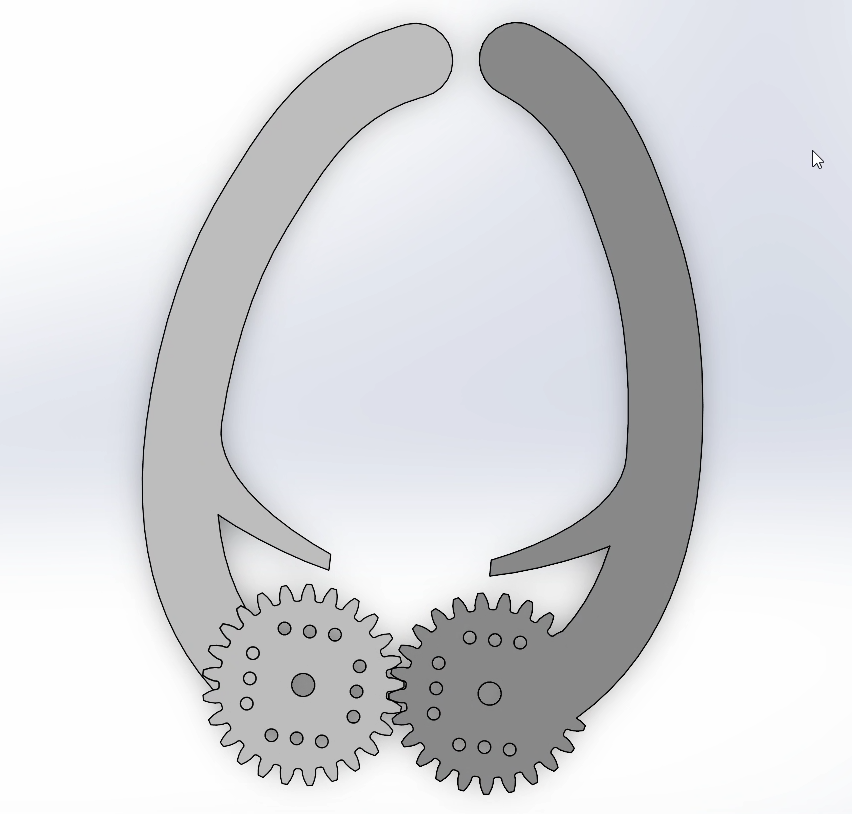
\includegraphics[width=\linewidth]{gripper_cad.png}
    \caption{Jaws and gear pair in CAD}
  \end{subfigure}\hfill
  \begin{subfigure}[b]{0.64\linewidth}
    \centering
    \begin{tikzpicture}[scale=1.35]
      % parabola x = y^2/(4f) with f = 1, drawn with the travel direction upward
      \draw[ink, line width=1.2pt, domain=-2.6:2.6, samples=60] plot (\x,{\x*\x/4});
      \draw[dashed, draw=ink!55] (0,-0.3) -- (0,2.6);
      \fill[ink] (0,1) circle (1.2pt);
      \node[note, anchor=east] at (-0.1,1.0) {focus};
      % contact point at y = 1.8, inward unit normal (-0.669, 0.743)
      \coordinate (P) at (1.8,0.81);
      \draw[draw=cA, fill=cA!18] ($(P)+(-0.368,0.409)$) circle (0.55);
      \node[note, text=cA] at ($(P)+(-0.368,0.409)$) {coin};
      \draw[->, cB, line width=0.8pt] (P) -- ($(P)+(-1.07,1.19)$);
      \node[note, text=cB, anchor=south] at ($(P)+(-1.07,1.19)$) {normal force};
      % tangent and the direction of travel through the contact point
      \draw[draw=ink!55] (P) -- ($(P)+(0.89,0.80)$);
      \draw[draw=ink!55] (P) -- ($(P)+(0,1.2)$);
      \draw[draw=ink] ($(P)+(0,0.75)$) arc (90:42:0.75);
      \node[note] at ($(P)+(0.3,0.95)$) {$\alpha$};
      \draw[->, line width=0.8pt] (-2.9,0.2) -- (-2.9,1.2);
      \node[note, anchor=north] at (-2.9,0.15) {travel};
      \draw[->] (0.6,-0.3) -- (1.4,-0.3);
      \node[note, anchor=west] at (1.45,-0.3) {$y$};
    \end{tikzpicture}
    \caption{A coin in contact with a parabolic jaw}
  \end{subfigure}
  \caption{The gripper. A coin touched by a jaw is pushed along the normal of the profile,
  which has an inward component everywhere except at the vertex.}
  \label{fig:gripper}
\end{figure}

The mechanics of this can be stated simply (\cref{fig:gripper}b). Let the profile be the
parabola $y^2=4fx$ with focal length $f$, opening in the direction of travel, and let the
robot advance onto a coin that lies at a lateral offset $y$ from the axis. The jaw meets the
coin with a surface inclined at an angle $\alpha$ to the direction of travel, where
\begin{equation}
  \tan\alpha = \frac{\mathrm{d}y}{\mathrm{d}x} = \frac{2f}{y}.
\end{equation}
The contact force lies within the friction angle $\varphi=\arctan\mu$ of the surface normal.
The coin slides along the jaw, towards the axis, as long as the direction of travel lies
outside that friction cone, that is, as long as $90^\circ-\alpha>\varphi$. With
$\tan\alpha=2f/y$ this gives
\begin{equation}
  \lvert y\rvert > 2\mu f .
  \label{eq:centring}
\end{equation}
A coin that meets the jaw further from the axis than $2\mu f$ is carried inward; inside
that band friction is able to hold it where it is. Two conclusions follow. The centring
improves with a short focal length and a slippery jaw, and the tips of the jaws, where
$\alpha$ is small, are where it works best, which is where a misaligned approach makes
first contact. For the friction coefficient of 0.35 used for the coin in the simulation, the
band is $0.7f$ on either side of the axis. I have not measured the focal length of the
printed jaws, and \cref{eq:centring} is given as the design rule and not as a verified
figure. When the jaws close, the coin is centred in any case, since the closed jaws leave it
little room.

\subsubsection{Release Ridges}
Each jaw carries a ridge on its inner side, near the pivot (\cref{fig:gripper}a). When the
jaws open, the ridges swing forward and push the coin out of the throat. Without them a coin
could stay against the gears as the robot backs away and be drawn back with it. With them
the coin is left where it was released. This detail decided whether a coin placed in a bin
stayed there.

\subsubsection{Actuation}
One MG995 servo drives the gripper. Its shaft turns one jaw directly, and a pair of involute
gears with equal numbers of teeth turns the other jaw by the same angle in the opposite
sense. The pivots are 25\unit{mm} apart, so each gear has a pitch diameter of 25\unit{mm}.
An involute profile keeps the velocity ratio constant through the mesh~\cite{shigley},
and equal gears make the motion of the two jaws symmetrical without any linkage.

At 4.8\unit{V} the servo is rated at 8.5\unit{kg\,cm}, which is 0.83\unit{N\,m}, and at
$60^\circ$ in 0.20\unit{s}, which is 5.2\unit{rad/s}. At the tip of a jaw, 90\unit{mm} from
the pivot, the stall torque corresponds to a force of 9\unit{N}, two orders of magnitude
above the 0.08\unit{N} needed to slide a coin. The jaws travel between an open position at
$-1.0\unit{rad}$ and a closed position at $0.09\unit{rad}$ of the driven jaw; the jaws touch
one another at about $0.096\unit{rad}$. The stroke of 1.09\unit{rad} takes 0.21\unit{s} at
the rated speed, and the mission software allows one second for it. In the pose in which the
assembly was exported, the second jaw is $7.25^\circ$ away from the mirror image of the
first, so the jaws meet slightly to one side of the centre line. This is an error of
assembly in the CAD model that the simulation reproduces.

\subsection{Sensor Placement}
\label{sec:sensors-mech}
\subsubsection{Depth Camera}
The camera looks forward from a height of 85\unit{mm}. Its depth image has a vertical field
of view of $58^\circ$, so the lowest ray leaves the lens $29^\circ$ below the horizontal and
reaches the floor at a distance
\begin{equation}
  x_{\min} = \frac{h_c}{\tan 29^\circ} = \frac{85\unit{mm}}{0.554} \approx 0.15\unit{m}
  \label{eq:blind}
\end{equation}
ahead of the lens (\cref{fig:blind}). Depth is in addition not reported below a range of
0.2\unit{m}. A caged coin lies about 4\unit{cm} ahead of the lens. The camera therefore
never sees the coin it is about to pick, nor the last 15\unit{cm} of floor in front of the
robot. This is the most important constraint that the mechanical design places on the
software, and \cref{sec:docking} describes how the infrared array takes over where the
camera ends.

\begin{figure}[htbp]
  \centering
  \begin{tikzpicture}[scale=0.38]
    % units: 10 mm, side view. Lens at x = 14.2, height 8.5.
    \draw[draw=ink] (-4,0) -- (36,0);
    % chassis plate and wheel
    \draw[draw=ink, fill=panel] (-1.7,2.7) rectangle (16.3,3.3);
    \draw[draw=ink, fill=white] (0,2.2) circle (2.2);
    % camera post and body
    \draw[draw=ink, fill=white] (12.0,3.3) rectangle (13.0,7.2);
    \draw[draw=ink, fill=ink!70] (11.7,7.2) rectangle (14.2,9.7);
    % field of view
    \fill[cA!14] (14.2,8.5) -- (29.53,0) -- (36,0) -- (36,13.5) -- (23.2,13.5) -- cycle;
    \draw[cA] (14.2,8.5) -- (29.53,0);
    \draw[cA] (14.2,8.5) -- (23.2,13.5);
    \draw[dashed, draw=ink!55] (14.2,8.5) -- (24,8.5);
    \draw[draw=ink] (19.2,8.5) arc (0:-29:5);
    \node[note] at (21.0,7.1) {$29^\circ$};
    % blind zone
    \draw[cB, line width=1.6pt] (14.2,0) -- (29.53,0);
    \draw[|-|] (14.2,-1.2) -- (29.53,-1.2);
    \node[note, below] at (21.9,-1.3) {0.15\,m not seen};
    % coin
    \draw[draw=cB, fill=cB!25] (15.8,0) rectangle (19.8,1.5);
    \node[note, text=cB, anchor=south] at (17.8,1.7) {caged coin};
    % jaws
    \draw[draw=ink, fill=white] (12.0,0.82) rectangle (21.0,1.62);
    % IR array
    \draw[draw=ink, fill=white] (3.5,0.74) rectangle (6.1,2.7);
    \node[note, anchor=north] at (4.8,-0.1) {IR array};
    % height
    \draw[|-|] (9.6,0) -- (9.6,8.5);
    \node[note, anchor=east] at (9.5,5.4) {85\,mm};
    \node[note, text=cA] at (31.5,7.5) {field of view};
  \end{tikzpicture}
  \caption{Side view of the front of the robot, to scale. The floor closer than 0.15\unit{m}
  to the lens is below the field of view of the depth camera, and so is a coin between the
  jaws.}
  \label{fig:blind}
\end{figure}

The holder places the camera 54\unit{mm} to the left of the centre line, beside the servo.
The offset is known to the software through the robot description, so it does not bias the
map, but it is the cause of the lateral shift of the centre of mass found in \cref{sec:mass}.

\subsubsection{Infrared Array}
The array has eight reflectance channels in a row across the robot, 15\unit{mm} apart, which
gives it a span of 105\unit{mm} between the outer channels. Its sensing face is 7.4\unit{mm}
above the floor. Two properties of its position matter later. It is 48\unit{mm} ahead of the
axle, and this distance acts as a look-ahead that damps the line follower
(\cref{sec:linefollower}). And it is 72\unit{mm} behind the gripper pivots, so that a marking
on the floor under the array fixes the position of the jaws relative to that marking; the
pick and drop markings of the arena are placed accordingly (\cref{sec:arena}).

\subsection{Manufacture}
\label{sec:manufacture}
The chassis, the jaws, the gears and the camera holder are printed in PLA. Holes and
pockets were toleranced for the bolts and nuts in use, and the chassis was printed in more
than four iterations to find clearances that the printer reproduced. All bolts have
hexagon socket heads, which take a higher tightening torque from a key than a slotted or
cross head does from a screwdriver and are standard in prototype work.
